\section{Methodology}

\begin{figure}[!ht]
    \hspace*{-0.7cm} 
    \subfloat[Informer Architecture\label{fig:informer}]{%
      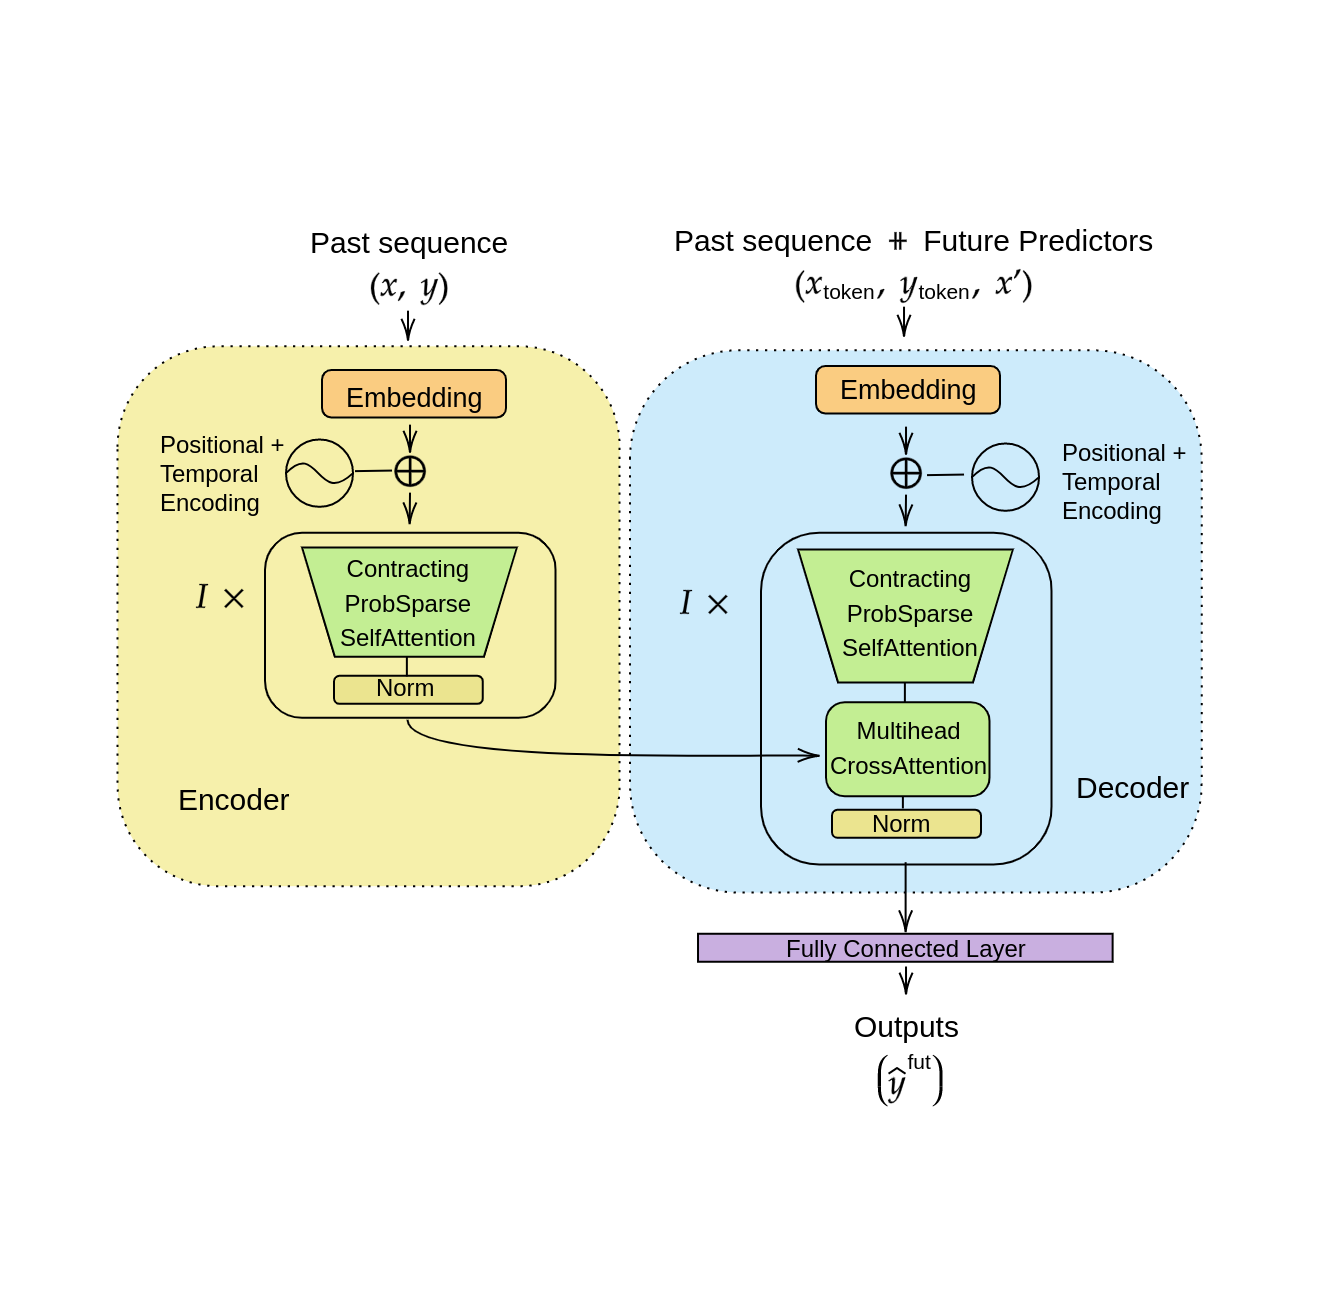
\includegraphics[width=0.55\textwidth]{figs/informer_new.png}
    }
    \subfloat[Yformer Architecture\label{fig:Yformer}]{%
      \includegraphics[width=0.45\textwidth]{figs/YFormerv2.png}
    }
\caption{Comparison of Informer and Yformer architecture highlighting the three key differences. (1) The Informer architecture process part of the past input data $(x, y)$ within the decoder as $(x_{\text{token}}, y_{\text{token}})$ along with the future predictors $(x')$. The Yformer avoids this redundant reprocessing of $(x,y)$ and uses a masked self-attention network for embedding the only the future predictors $(x')$. (2) The Informer uses the final encoder embedding as the input to the decoder. The Yformer passes a concatenated ( $\doubleplus$) representation ($e_i$) of the $i^{\text{th}}$ Y-Past and Y-Future Encoder embedding to the ${I-i}^{th}$ layer of the Y-Decoder, forming a U-Net connection (represented in red) between the encoder and the decoder. (3) The Yformer architecture predicts both the input reconstruction $\hat{y}^{\text{past}}$ and future predictions $\hat{y}^{\text{fut}}$.}
\label{fig:architecture}
\end{figure}


The Yformer model is a Y-shaped symmetric encoder-decoder architecture that is specifically designed to take advantage of the multi-resolution embeddings generated by the \textsl{Contracting ProbSparse Self-Attention Blocks}. The fundamental design consideration is the adoption of U-Net-inspired connections to extract encoder features at multiple resolutions and provide a direct connection to the corresponding symmetric decoder block. The Yformer additionally utilizes reconstruction loss to learn generalized embeddings that better approximate the data generating distribution. Figures \ref{fig:informer} and \ref{fig:Yformer} compares the Informer architecture with the Yformer and Figure \ref{fig:unet} illustrates the U-Net connections employed by the Yformer model.

The \textbf{Y-Past Encoder} of the Yformer is designed using a similar encoder structure as that of the Informer (Figure \ref{fig:informer}). The Y-Past Encoder embeds the past sequence $(x, y)$ into a scalar projection along with the addition of positional and temporal embeddings. Multiple \textsl{Contracting ProbSparse Self-Attention Blocks} are used to generate encoder embeddings at various resolutions following a contracting pyramid structure. The Informer model uses the final low-dimensional embedding as the input to the decoder whereas, the Yformer retains the embeddings at multiple resolutions to be passed on to the decoder. This allows the Yformer to use high-dimensional lower-level embeddings effectively.

The \textbf{Y-Future Encoder} of the Yformer mitigates the redundant reprocessing of the past sequence $(x,y)$ (used as tokens $(x_{\text{token}}, y_{\text{token}})$ in the Informer architecture) by passing only the future predictors $(x')$ through the Y-Future Encoder and utilizing the multi-resolution embeddings to dismiss the need for tokens entirely. The attention blocks in the Y-Future encoder are based on a masked canonical self-attention mechanism \cite{vaswani2017attention} to prevent any information leak from the future time steps into the past. Thus, the Y-Future Encoder is designed by stacking multiple \textsl{Contracting ProbSparse Self-Attention Blocks} where the \textsl{ProbSparse} attention is replaced by the \textsl{Masked Attention}. We name these blocks \textsl{Contracting Masked Self-Attention Blocks}.

The Yformer processes the past inputs and the future predictors separately within its encoders. However, considering the time steps, the future predictors are a continuation of the past time steps. For this reason, the Yformer model concatenates ( represented by the symbol $\doubleplus$) the past encoder embedding and the future encoder embedding along the time dimension after each encoder block, preserving the continuity between the past input time steps and the future time steps. Let $i$ represent the index of an encoder block, then $e^{\text{past}}_{i+1}$ and $e^{\text{fut}}_{i+1}$ represent the output from the past encoder and the future encoder respectively. The final concatenated encoder embedding $(e_{i+1})$ is calculated as, 

\begin{equation}
\begin{aligned}
    e^{\text{past}}_{i+1} &= \operatorname{ContractingProbSparseSelfAttentionBlock}(e^{\text{past}}_{i}) \\
    e^{\text{fut}}_{i+1} &= \operatorname{ContractingMaskedSelfAttentionBlock}(e^{\text{fut}}_{i}) \\
    e_{i+1} &= e^{\text{past}}_{i+1} \doubleplus e^{\text{fut}}_{i+1}
    \label{Eq:concatencoders}
\end{aligned}
\end{equation}
The encoder embeddings represented by $\mathcal{E} = [e_0, \dots, e_{I}]$ (where $I$ is the number of encoder layers) contain the combination of past and future embeddings at multiple resolutions.

The \textbf{Y-Decoder} of the Yformer consists of two parts. The first part takes as input the final concatenated low-dimensional embedding $(e_I)$ of the encoders and performs a multi-head canonical self-attention mechanism. Since the canonical self-attention layer is separated from the repeating attention blocks within the decoder, the Yformer complexity from this full attention module does not increase with an increase in the number of decoder blocks. The U-Net architecture inspires the second part of the Y-Decoder. Consequently, the decoder is structured in a symmetric expanding path identical to the contracting encoder (Figure \ref{fig:unet}). We realize this idea by introducing  \textsl{Expanding ProbSparse Cross-Attention Block} for symmetric upsampling.

\begin{figure}[t]
 \centering
 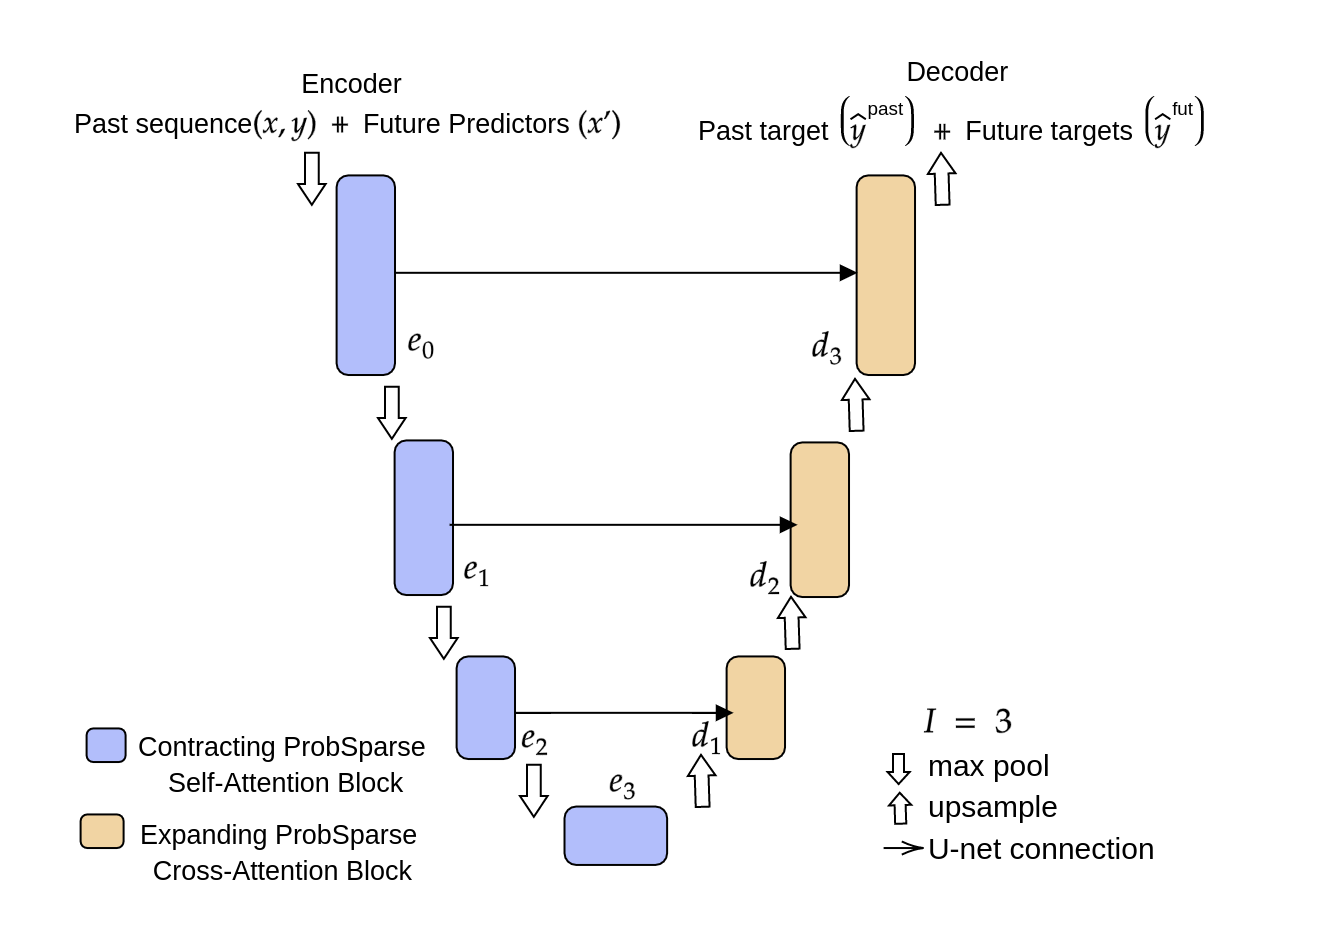
\includegraphics[width=0.6\textwidth]{figs/unet_yformer.png}
 \caption{U-Net connections for effectively utilizing embeddings at multiple resolutions in the Yformer. The 
 Y-Past Encoder embeddings and the Y-Future Encoder embeddings are concatenated within the Yformer encoder. A direct connection is allowed between the contracting encoder embedding $(e_i)$ and the corresponding expanding decoder embedding $(d_{I-i})$. ($\doubleplus$ denotes concatenation) }
 \label{fig:unet}
\end{figure}

The \textbf{\textsl{Expanding ProbSparse Cross-Attention Block}} within the Yformer decoder performs two tasks: (1) upsample the compressed encoder embedding $e_I$ and (2) perform restricted cross attention between the expanding decoder embedding $d_{I-i}$ and the corresponding encoder embedding $e_i$ as shown below. 
% \squeezeup
\begin{algorithm}[H]
    \textit{Input}  : $d_{I-i}, e_i$  \\
    \textit{Output} : $d_{I-i+1}$\\
    $d_{I-i+1} \gets \operatorname{ProbSparseCrossAttn} (d_{I-i}, e_i)$ \\
    $d_{I-i+1} \gets \operatorname{Conv1d} (d_{I-i+1})$\\
    $d_{I-i+1} \gets \operatorname{LayerNorm} (d_{I-i+1})$ \\
    $d_{I-i+1} \gets \operatorname{ELU}(\operatorname{ConvTranspose1d} (d_{I-i+1})))$
 \caption{Expanding ProbSparse Cross-Attention Block}
\end{algorithm}


The \textsl{Expanding ProbSparse Cross-Attention Blocks} within the Yformer decoder uses a $\operatorname{ProbSparseCrossAttn}$ to construct direct connections between the lower levels of the encoder and the corresponding symmetric higher levels of the decoder. Direct connections from the encoder to the decoder are an essential component for the majority of models within the image domain. For example, ResNet \cite{he2016deep}, and DenseNet \cite{huang2017densely} have demonstrated that direct connections between previous feature maps, strengthen feature propagation, reduce parameters, mitigate vanishing gradients and encourage feature reuse. However, current transformer-based architectures fail to utilize these direct connections.  

We utilize $\operatorname{ConvTranspose1d}$ or popularly known as $\operatorname{Deconvolution}$ for incrementally increasing the embedding space. The famous U-Net architecture uses a symmetric expanding path using such $\operatorname{Deconvolution}$ layers. This property enables the model to not only aggregate over the input but also upscale the latent dimensions, improving the overall expressivity of the architecture. The decoder of Yformer follows a similar strategy by employing $\operatorname{Deconvolution}$ to expand the embedding space of the encoded output as shown in Figure \ref{fig:unet}.

Finally, a fully connected layer ($\operatorname{LinearLayer}$) predicts the future time steps $\hat{y}^{\text{fut}}$ from the  final decoder layer $(d_I)$ and additionally reconstructs the past input targets $\hat{y}^{\text{past}}$ for the reconstruction auxiliary loss.

\begin{equation}
    \begin{aligned}
        {[\hat{y}^{\text{past}}, \hat{y}^{\text{fut}}]} &= \operatorname{LinearLayer} (d_I) \\
    \end{aligned}
    \label{eqn:prediction}
\end{equation}

The addition of reconstruction loss to the Yformer as an auxiliary loss serves two significant purposes. Firstly, the reconstruction loss acts as a data-dependent regularization term that reduces overfitting by learning embeddings that are more general \cite{Jarrett2020Target-Embedding}. Secondly, the reconstruction loss helps in producing future output in a similar distribution as the inputs. For far horizon forecasting, we are interested in learning a future-output distribution, however, the future-output distribution and the past-input distribution arise from the same data generating process. Therefore having an auxiliary reconstruction loss would direct the gradients to a better approximate of the data generating process. Consequently, the Yformer model is trained on the combined loss $\ell$, 

\begin{equation}
    \ell = \alpha \, \ell^{\text{mse}}(y, \hat{y}^{\text{past}}) + (1-\alpha) \, \ell^{\text{mse}}(y', \hat{y}^{\text{fut}}) 
    \label{eqn:reconstruction}
\end{equation}
where the first term tries to learn the past targets $y$ and the second term learns the future targets $y'$. We use the reconstruction factor $(\alpha)$ to vary the importance of reconstruction and future prediction and tune this as a hyperparameter. 
